\vspace{-5pt}
Desde hace pocos años, el Análisis de Redes Sociales (o SNA por sus siglas en inglés de Social Network Analysis) ha contribuido a las investigaciones criminales y a las actividades de inteligencia relacionadas.
Actualmente los organismos estatales encargados de la Justicia y la prevención del delito cuentan con registros informatizados de las actividades criminales detectadas, así como de las etapas y eventos del subsecuente proceso penal. 
Esta información constituye en esencia, una red social. 
Para este trabajo es de especial interés la información producida por las fuerzas policiales de la Provincia del Chubut y su Poder Judicial de la mano del Ministerio Público Fiscal (MPF). 

Coirón es el sistema informático que colabora con la administración del flujo de casos ingresados al MPF~\cite{MPFChubutPaginaWeb}. Es una herramienta que permite registrar, comunicar y gestionar las actividades, trámites y actuaciones que se realizan para un caso penal, desde la denuncia hasta su finalización. También es una herramienta de administración de información, flujo de casos, planificación, organización, coordinación y control.
Ha sido desarrollado a medida de las necesidades del MPF, adaptado al Código Procesal Penal vigente y a los lineamientos estratégicos definidos. Su progreso, mantenimiento y mejora continua está a cargo del Equipo de Desarrollo del Departamento de Informática del Área de Planificación y Control de Gestión de la Procuración General.
Actualmente nos encontramos trabajando en la incorporación de herramientas de visualización de información, potenciando el análisis que realizarán luego los especialistas de análisis criminal.
Se denomina "Grupo de Pertenencia" en el Sistema Coirón a la relación directa que existe entre un individuo dentro del universo de personas cargadas como actores de delitos (roles: denunciado, sospechoso o imputado) y otros individuos del mismo universo, con los cuales existan uno o más casos penales en común.
Crear un módulo de software "Red de Grupos de Pertenencia" donde se muestre gráficamente las relaciones entre las personas involucradas en los casos penales es el objetivo principal de esta investigación. No sólo enfocarse en el grupo de pertenencia de una persona en particular, sino que mediante herramientas inteligentes, una visualización y con diversos filtros de búsqueda, se logre mostrar gráficamente las relaciones entre un determinado grupo de personas y de esta manera poder inferir la conformación de posibles bandas delictivas.
La idea central modelar mediante un grafo los grupos de pertenencia. Dentro del mismo se le llamará nodo a cada círculo, y representa a una persona (con los roles ya mencionados) involucrada en dos o más casos penales. Existe un gran cúmulo de personas en el sistema con sólo un caso con rol de denunciado, por esa razón se los excluye del universo a analizar, no obstante podrían ser parte del dataset a visualizar si alguno/s de ellos se encuentran relacionados con otros nodos del primer grupo. El tamaño del nodo posee una relación directa con la cantidad de casos penales en los que se encuentre involucrada la persona. Cuanto mayor sea el tamaño del nodo en más cantidad de casos penales estará involucrado.
Los arcos entre pares de nodos, vinculan a las personas entre sí y representan el o los casos que tienen en común. El grosor de la vinculación será directamente proporcional a la cantidad de casos en común entre un par de personas. Hay nodos que se encontrarán aislados en el grafo, esto no significa que no estén involucrados en casos, sino que quizás no existan relaciones para el filtro de búsqueda que se utilice en esa vista en particular.

Supongamos que una persona "A" se encuentra asociada a 8 casos penales, una persona "B" a 4 y una persona "C" a 2 casos. Agreguemos que las personas "A" y "B" se encuentran relacionadas entre sí, por estar en 3 casos en común (casos 1, 2 y 3). Por otro lado las personas "A" y "C" también se encuentran relacionadas, por tener un caso en común (caso 4).  Una representación gráfica de dicha situación se muestra en la Figura \ref{fig:grafode2}, y puede observarse el doble de tamaño entre el nodo "A" y el nodo "B", representando justamente la diferencia de casos entre ambos nodos (8 y 4 casos). También se ve a simple vista el grosor del enlace entre "A" y "B" tres veces más grande que el enlace entre "A" y "C" (3 casos en común entre el primer par de nodos, y sólo un caso para el último par de nodos mencionado). 
\vspace{-15pt}
\begin{figure}
	\centering
	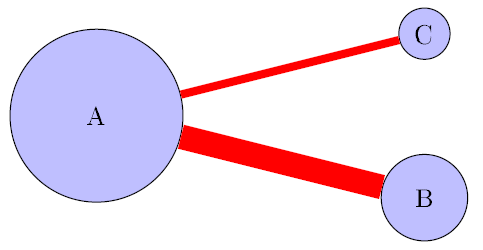
\includegraphics[width=0.25\linewidth]{grafo-ejemplo.png}
	\caption{Ejemplo de relación entre tres personas.} 
	\label{fig:grafode2}
\end{figure}
\vspace{-25pt}